\documentclass{article}
\usepackage{amssymb,amsmath, verbatim}
%\usepackage{titlesec}  
\usepackage{epsfig}
%\usepackage{placeins}
\usepackage[margin=2cm]{geometry}
%\usepackage{fancyhdr}
%\pagestyle{fancy}
%\renewcommand{\headrulewidth}{0pt}
%\renewcommand{\footrulewidth}{1pt}

\usepackage{graphicx}
\usepackage[T1]{fontenc}
\usepackage{listings}
\usepackage{bm}

%\usepackage{names}

\DeclareMathOperator*{\argmax}{\arg\!\max}
\DeclareMathOperator*{\argmin}{\arg\!\min}

\newcommand{\pdiff}[2]{
        \frac{\partial #1}{\partial #2}
}

\newcommand{\diff}[2]{
        \frac{d #1}{d #2}
}


% Footer
%\lfoot{\thepage}
%\rfoot{\vspace{-.8cm} Nick Grunloh, Andrea Corredor, Abhinav Venkateswar Venkataraman
%\\\vspace{.14cm}
%\footnotesize grunloh@soe.ucsc.edu, acorredo@ucsc.edu, abhinav@soe.ucsc.eduu}


                 
%\titleformat{\subsection}[runin]{}{}{}{}[] % makes subsections not appear on their own lines


%Header
\newcommand{\header}[5]{
        \begin{minipage}[h!]{0.63\textwidth}
                \centering
                { \LARGE \textbf{ \textsc{#1} } }
        \end{minipage}
        \begin{minipage}[h!]{0.37\textwidth}
                \centering
                {#2}\\
                {#3}\\
        \end{minipage}
}

\begin{document}

\header{Machine Learning HW \#3}
       {Nick Grunloh\\Andrea Corredor\\Abhinav Venkateswar Venkataraman}
       {11/5/2013}
\\\\


\section{Linear Regression}

\subsection*{Training Set}
Running Weka's Linear Regression on the full training set we obtain the model below:

 \[ t =    -0.1343 * x_{1} +  1.8477 * x_{2}  -0.8966 * x_{3} + 4.3608 \]

\noindent And a root mean squared error of $0.1897$. 

\subsection*{Predicting $\hat{t}$}

\begin{align*}
 x = [3,3,5]  \\
 \hat{t} = -0.1343 * 3 +  1.8477 * 3 + -0.8966 * 5 + 4.3608  \\
\hat{t} = 5.018 
\end{align*}

\subsection*{Comparing weights}
Computing the weights using Bishop (3.34) $ w = (X^{T}X)^{-1}X^{T}t$  we obtain,

\[w = \begin{bmatrix}
       4.3608029  \\[0.3em]
       -0.1342938  \\[0.3em]
       1.8476838 \\[0.3em]
       -0.8965848
     \end{bmatrix} \]

These weights are essentially identical to the ones computed by Weka's Linear Regression, except that Weka's have been rounded to $4^{th}$ decimal place.

\subsection*{Permuting the rows of $X$}
Reordering the examples has no impact on the weights computed with Bishop (3.34)
\[w_{reordered} = \begin{bmatrix}
       4.3608029  \\[0.3em]
       -0.1342938  \\[0.3em]
       1.8476838 \\[0.3em]
       -0.8965848
     \end{bmatrix} \]

It also did not affect the result of Weka's Linear Regression, which remained exactly the same as those of \mbox{part a}. 

\section{Interaction of sample size with the prior}

\begin{align*}
E_{\text{total}} = \frac{1}{2} \sum_{n=1}^{N}\left(  t_{n} - w^{T}\phi\left( x_{n}\right)  \right)^{2} + \frac{\lambda}{2}w^{T} w  
\end{align*}
$N$ training points all with $\phi\left( x_{n} \right) = 1$ and $t_{n} = 10$

\subsection*{Part a: Minimizing $w$}

\begin{align*}
E_{\text{total}} = \frac{1}{2} \sum_{n=1}^{N}\left( 10 - w^{T} 1 \right)^{2} + \frac{\lambda}{2}w^{T} w  \\
w^{T} = w  \Rightarrow w^{T}w = w^{2} \\
E_{\text{total}} = \frac{1}{2} \sum_{n=1}^{N}\left( 10 - w \right)^{2} + \frac{\lambda}{2}w^{2} \\
E_{\text{total}} = \frac{1}{2} \left( 10 - w \right)^{2}N + \frac{\lambda}{2}w^{2} \\
\frac{\text{d}E}{\text{d}w} = -N\left( 10 -w \right) + \lambda w = 0 \\
w\left( \lambda + N \right) = 10N \\
w = \frac{10N}{\lambda + N}
\end{align*}

\subsection*{Part b}
For what value of $\lambda$ (as a function of $N$) is the minimizing $w = 5$ ?
\begin{align*}
5 = \frac{10N}{\lambda + N} \\
\lambda + N = 2N \\
\lambda = N
\end{align*}
For fixed $\lambda$, what happens to the minimizing $w$ as $N$ goes to infinity?
\begin{align*}
w = \lim_{N \rightarrow \infty} \frac{10N}{\lambda + N} \\
w = \lim_{N \rightarrow \infty} \frac{10}{\frac{\lambda}{N} + 1} \\
\Rightarrow w = 10
\end{align*}



\section{Logistic Regression}
\begin{align*}
p(1|\bm{x},~\bm{w}) &= \frac{ \exp\left\{ \bm{x}'\bm{w} \right\} }{ 1+\exp\left\{ \bm{x}'\bm{w} \right\} }\\
p(0|\bm{x},~\bm{w}) &= 1-p(1|\bm{x},~\bm{w})\\
		    &= \left(\frac{1+ \exp\left\{ \bm{x}'\bm{w} \right\} }{ 1+\exp\left\{ \bm{x}'\bm{w} \right\} }\right)-\left(\frac{ \exp\left\{ \bm{x}'\bm{w} \right\} }{ 1+\exp\left\{ \bm{x}'\bm{w} \right\} }\right)\\
		    &= \frac{ 1 }{ 1+\exp\left\{ \bm{x}'\bm{w} \right\} }\\
		    &\nonumber\\
\ln\left\{ \frac{p(1|\bm{x},~\bm{w})}{p(0|\bm{x},~\bm{w})} \right\} &= \ln \left\{ 
	\frac{ \frac{ \exp\left\{ \bm{x}'\bm{w} \right\} }{ 1+\exp\left\{ \bm{x}'\bm{w} \right\} } }
	     { \frac{ 1 }{ 1+\exp\left\{ \bm{x}'\bm{w} \right\} } } 
	\right\}\\
		    &= \ln\left\{ \exp\left\{ \bm{x}'\bm{w} \right\} \right\}\\
		    &= \bm{x}'\bm{w}~=~\bm{w}'\bm{x}
\end{align*}

\section{Gradient of the cross-entropy error}
\begin{align*}
y_n &= \sigma(\bm{x}_{i}^{T}\bm{w})=\frac{\exp\left\{ a \right\}}{\left( 1+\exp\left\{ a\right\} \right)}\\
&\nonumber\\
\diff{\sigma(a)}{a} &= \diff{\exp\left\{ a \right\} \left( 1+\exp\left\{ a\right\} \right)^{-1}}{a}\\
		    &= \frac{\exp\left\{ a \right\}}{\left( 1+\exp\left\{ a\right\} \right)} -
		       \left( 
			\frac{\exp\left\{ a \right\}}{\left( 1+\exp\left\{ a\right\} \right)}
		       \right)
		       \left(
			\frac{\exp\left\{ a \right\}}{\left( 1+\exp\left\{ a\right\} \right)}
		       \right)\\
		    &= \sigma(a)\left(1-\sigma(a)\right)\\
&\nonumber\\
E(\bm{w}) &= -\sum_{i=1}^N t_i \ln\left\{ \sigma(\bm{x}_{i}^{T} \bm{w}) \right\} + (1-t_i)\ln\left\{1-\sigma(\bm{x}_{i}^{T}\bm{w})\right\}\\
\nabla_{\bm{w}} E(\bm{w}) &= -\nabla_{\bm{w}}\left[\sum_{i=1}^N t_i \ln\left\{ \sigma(\bm{x}_{i}^{T}\bm{w}) \right\} + (1-t_i)\ln\left\{1-\sigma(\bm{x}_{i}^{T}\bm{w})\right\}\right]\\
&=-\sum_{i=1}^N t_i \frac{1}{\sigma} \sigma(1-\sigma)\bm{x}_{i} + (1-t_i) \frac{1}{1-\sigma} \left(-\sigma(1-\sigma)\bm{x}_{i}\right)\\
&=\sum_{i=1}^{N} -t_i \bm{x}_{i} + t_i \sigma \bm{x}_{i} + \sigma \bm{x}_{i} - t_i \sigma \bm{x}_{i}\\
&=\sum_{i=1}^{N} (\sigma(\bm{x}_{i}^{T}\bm{w}) - t_i)\bm{x}_{i}
\end{align*}

\clearpage
\section{Perceptron algorithm with noise experiment}

\subsection*{Part a}
Epochs = 2
Prediction errors = 6

\subsection*{Part b}

%Epochs = 2
Prediction errors = 41

Would you expect it to take more or fewer epochs than part a? Why?

\begin{figure}[h!]
\centering
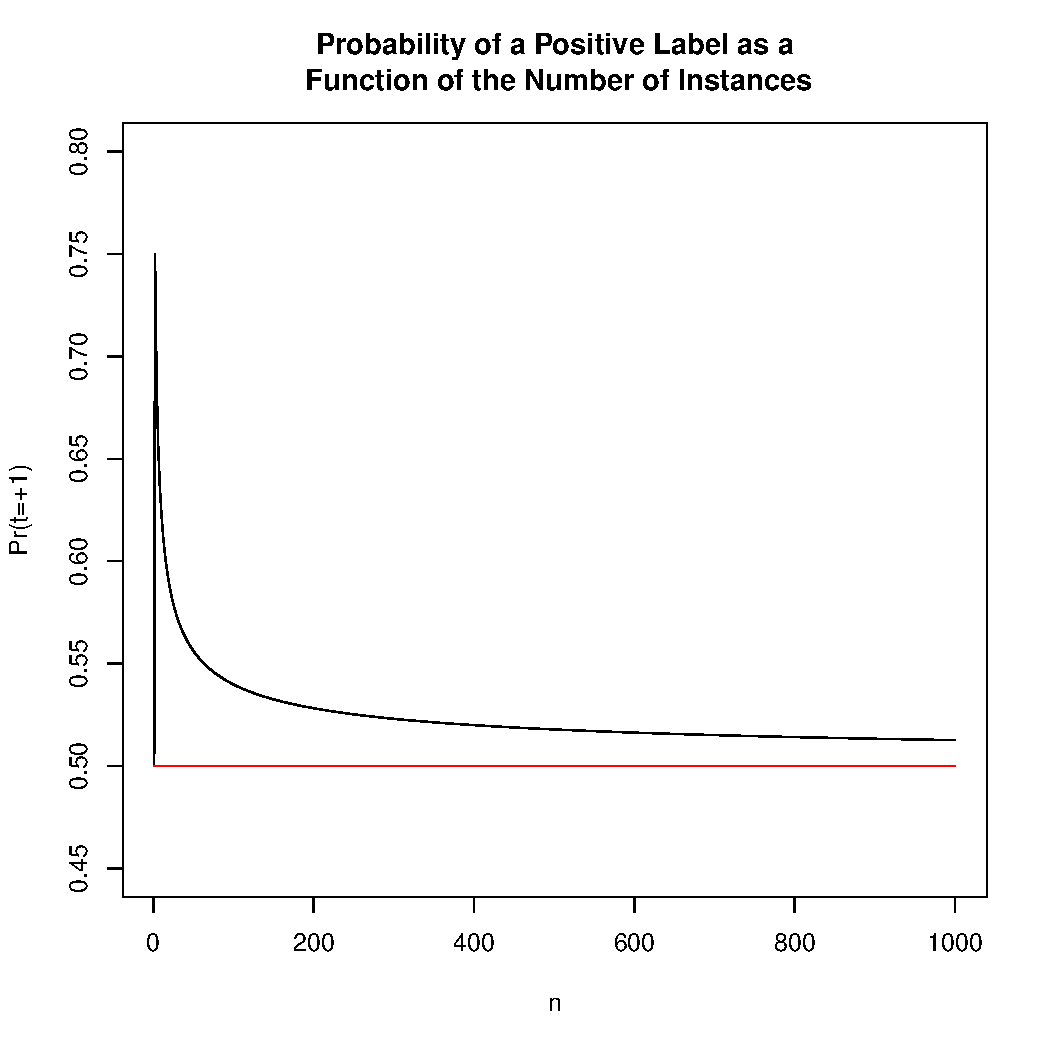
\includegraphics[width=0.8\textwidth]{bFig.pdf}
\caption{Since a $t=+1$ if at least $\frac{n}{2}$ of the instances of a given feature are $+1$, then the \mbox{$Pr(t=+1)=\sum_{i=\frac{n}{2}}^n Binomial(i|n,\frac{1}{2})$.}
The above graph is produced by evaluating this expression for \mbox{$n\in\left\{1,2,3,...,1000\right\}$.}
}
\label{bFig}
\end{figure}

Figure(\ref{bFig}) shows that $Pr(t=+1)$ increases above 0.5 (as it was in part a) and thus an example is more likely to be labeled $+$. 
Since $t$ is directly related to the way that we declare a mistake (ie. $(\bm{w\cdot x}_i) t_i \le0$), and the label generating mechanism increases how often $t=+1$ that will mean that more mistakes will occur per epoch because $\bm{w}$ and $\bm{x_i}$ are the same as before but $t_i=+1$ more often. % of the examples will be labeled.
%If we start with $w_0=\bm{0}$ then 
%The number of epochs could then increase because of the decrepency in the ratio $\frac{\#+}{\#-}$ could mean that the algorithm make worse and worse guesses in its learning process as it makes more mistakes. %this ratio is more and more skewed from 50/50.     
%The algorithm would converge more slowly because the guesses produced in each epoch could be much farther from valid separators due to the sw
For example consider the following graph that explores the relationship between $n$ and the average number of epochs, with all of the factors held the same.
Recall that when $1<n\le1000$ the $Pr(t=+1)>0.5$, especially when $n$ is small.
$Pr(t=+1)$ only converges to 0.5 as $n\rightarrow\infty$.

\begin{figure}[h!]
\centering
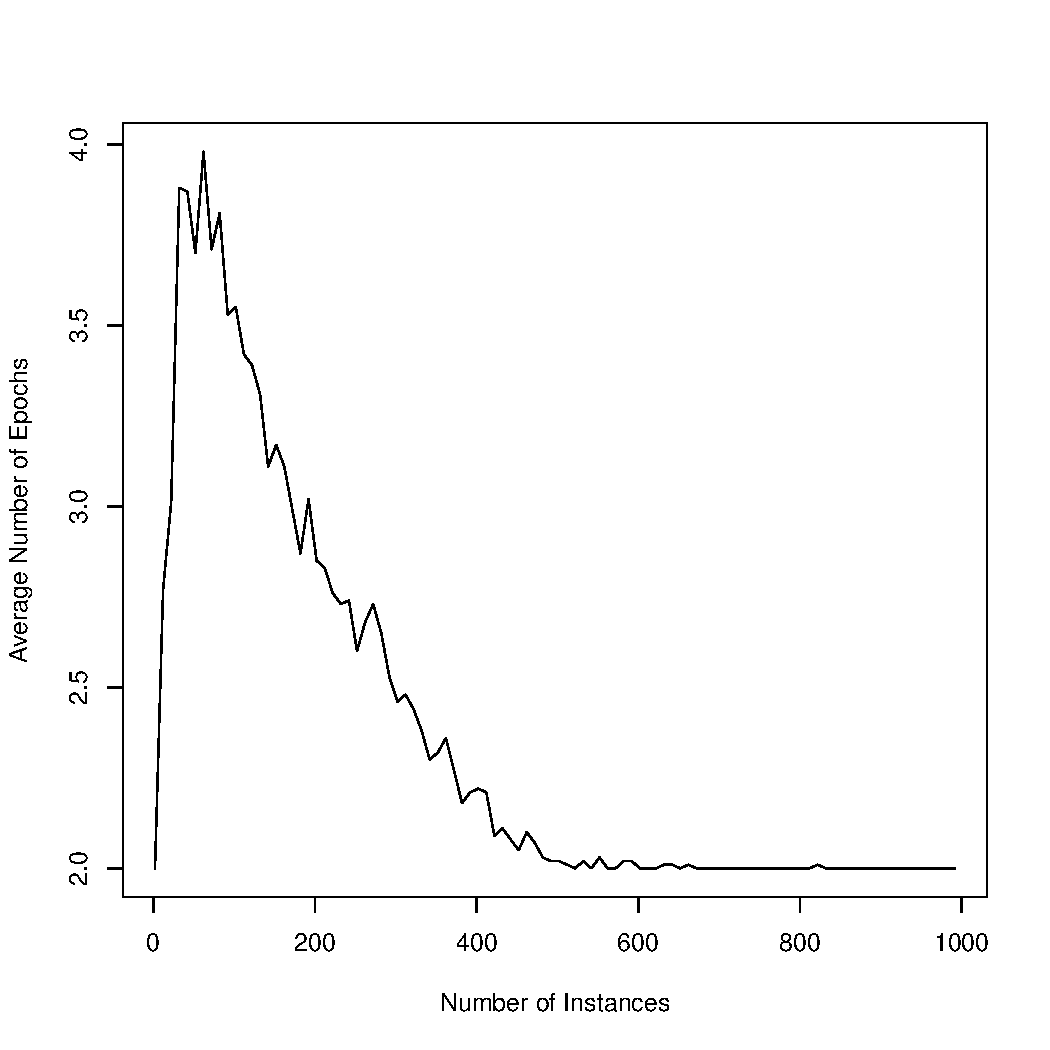
\includegraphics[width=0.8\textwidth]{epochsB.pdf}
%\caption{Since a $t=+1$ if at least $\frac{n}{2}$ of the instances of a given feature
%The above graph is produced by evaluating this expression for $n\in\left\{1,2,3,...,10
%}
\label{epoch}
\end{figure}

??? including the mistake rates from a and b for comparison would be great to support this theory. I'm not sure where these variables are being tracked can you add them easily Andrea?????



%I don't see why it would raise it. Does this have something to do with the gap?
%We expect it to take the same number of epochs, because the probability of being labeled plus is about the same as of being labeled minus (?). Quiver (?)

\clearpage
\subsection*{Part c}

Which of these will be more accurate on new unseen data? Create a separate test set (with the random noise) and evaluate the accuracy of these three hypotheses on it. Ambitious students may run this experiment multiple times (say 10)and report the average accuracies.
\\
Running the experiment 10 times: \\
Avg. accuracy for $w_{1000}$ = $0.7706$ \\
Avg. accuracy for $w_{avg}$ = $0.8384$ \\
Avg. accuracy for $w_{vote}$ = $0.8360$ \\

\noindent $w_{avg}$ and $w_{vote}$ are consistently superior to $w_{1000}$, with $w_{avg}$ slightly superior to $w_{vote}$.

\clearpage
\section{Appendix}


\verbatiminput{./perceptron.R}
\verbatiminput{./perceptron_partb.R}
\verbatiminput{./perceptron_partc.R}


\end{document}
